\documentclass[11pt]{article}

\usepackage[margin=1in]{geometry}
\usepackage[T1]{fontenc}
\usepackage{lmodern}
\usepackage{microtype}
\usepackage{amsmath,amssymb,amsthm,mathtools}
\usepackage{graphicx}
\usepackage[dvipsnames]{xcolor}
\usepackage{booktabs}
\usepackage{hyperref}

\hypersetup{
  colorlinks=true,
  linkcolor=MidnightBlue,
  citecolor=MidnightBlue,
  urlcolor=MidnightBlue
}

\newtheorem{theorem}{Theorem}
\newtheorem{proposition}{Proposition}
\newtheorem{corollary}{Corollary}
\newtheorem{remark}{Remark}

\newcommand{\E}{\mathbb{E}}
\newcommand{\Prob}{\mathbb{P}}
\newcommand{\Tmax}{T}

\title{\textbf{Eliminative Information in a Generalized Monty Hall Problem}\\
\large Increasing Marginal Value, Non-Myopic Search, and an Exact Cost Threshold}
\author{}
\date{}

\begin{document}
\maketitle

\begin{abstract}
The classical Monty Hall puzzle is usually presented as a one-step
probability paradox.  This note treats it instead as a small model of costly
information acquisition.  There are $K$ doors, $m$ prizes, and a knowledgeable
host who can sequentially reveal losing doors.  After paying for $t$ reveals,
the decision maker may switch uniformly to one of the still-closed doors
other than the initial choice.  The switch success probability is
\[
  S(t)=\frac{m(K-1)}{K(K-1-t)}.
\]
Because host reveals eliminate only losing doors, the marginal value
$S(t+1)-S(t)$ is strictly increasing.  Consequently the deterministic
stopping problem $\max_t\{S(t)-ct\}$ is not governed by a myopic rule.  Its
optimum is attained at an endpoint: either buy no information or buy all
available information.  The critical cost is exactly
\[
  c^*(K)=\frac1K,
\]
independent of the number of prizes $m$ whenever at least one reveal is
available.  Simulations and plots illustrate the resulting phase transition.
\end{abstract}

\section{From Puzzle to Information Acquisition}

The standard Monty Hall problem has three doors, one prize, one initial
choice, one host reveal, and one option to switch.  Its familiar answer,
``switching wins with probability $2/3$'', is not really about luck.  It is
about constrained information: the host knows where the prize is and is not
allowed to reveal it.

We generalize this mechanism.  A contestant faces $K$ doors, exactly $m$ of
which contain prizes, with $1\le m<K$.  The contestant first chooses one door
uniformly at random.  A host then reveals losing doors, never opening the
contestant's initial choice and never opening a prize.  Reveals are costly:
each reveal costs $c>0$.  After $t$ reveals, the contestant switches uniformly
to one of the remaining closed doors other than the initial choice.

The maximum number of possible reveals is
\[
  \Tmax=K-m-1.
\]
This is the number of losing doors not chosen by the contestant in the worst
case.  The feasible stopping times are therefore
\[
  t\in\{0,1,\dots,\Tmax\}.
\]

\paragraph{Key distinction.}
The host does not reveal prize values or sample new alternatives.  The host
only deletes impossible alternatives.  This is \emph{eliminative information}.
That distinction reverses the usual diminishing-returns intuition.

\section{\texorpdfstring{Switching After \(t\) Reveals}{Switching After t Reveals}}

\begin{theorem}[Switching probability]
After $t$ losing doors have been revealed, with $0\le t\le K-m-1$, the
probability of winning by switching uniformly among the available non-initial
doors is
\[
  S(t)=\frac{m(K-1)}{K(K-1-t)}.
\]
The probability of winning by staying is
\[
  S_{\mathrm{stay}}=\frac{m}{K}.
\]
\end{theorem}

\begin{proof}
Condition on whether the initial choice is a prize.  With probability $m/K$,
the initial door is a prize.  Then among the other $K-1-t$ closed switch
options, exactly $m-1$ are prizes.  With probability $(K-m)/K$, the initial
door is not a prize.  Then all $m$ prizes are among the $K-1-t$ switch
options.  Therefore
\[
  S(t)
  =
  \frac{m}{K}\frac{m-1}{K-1-t}
  +
  \frac{K-m}{K}\frac{m}{K-1-t}
  =
  \frac{m(K-1)}{K(K-1-t)}.
\]
Staying wins precisely when the initial choice was a prize, which has
probability $m/K$.
\end{proof}

\begin{figure}[ht]
  \centering
  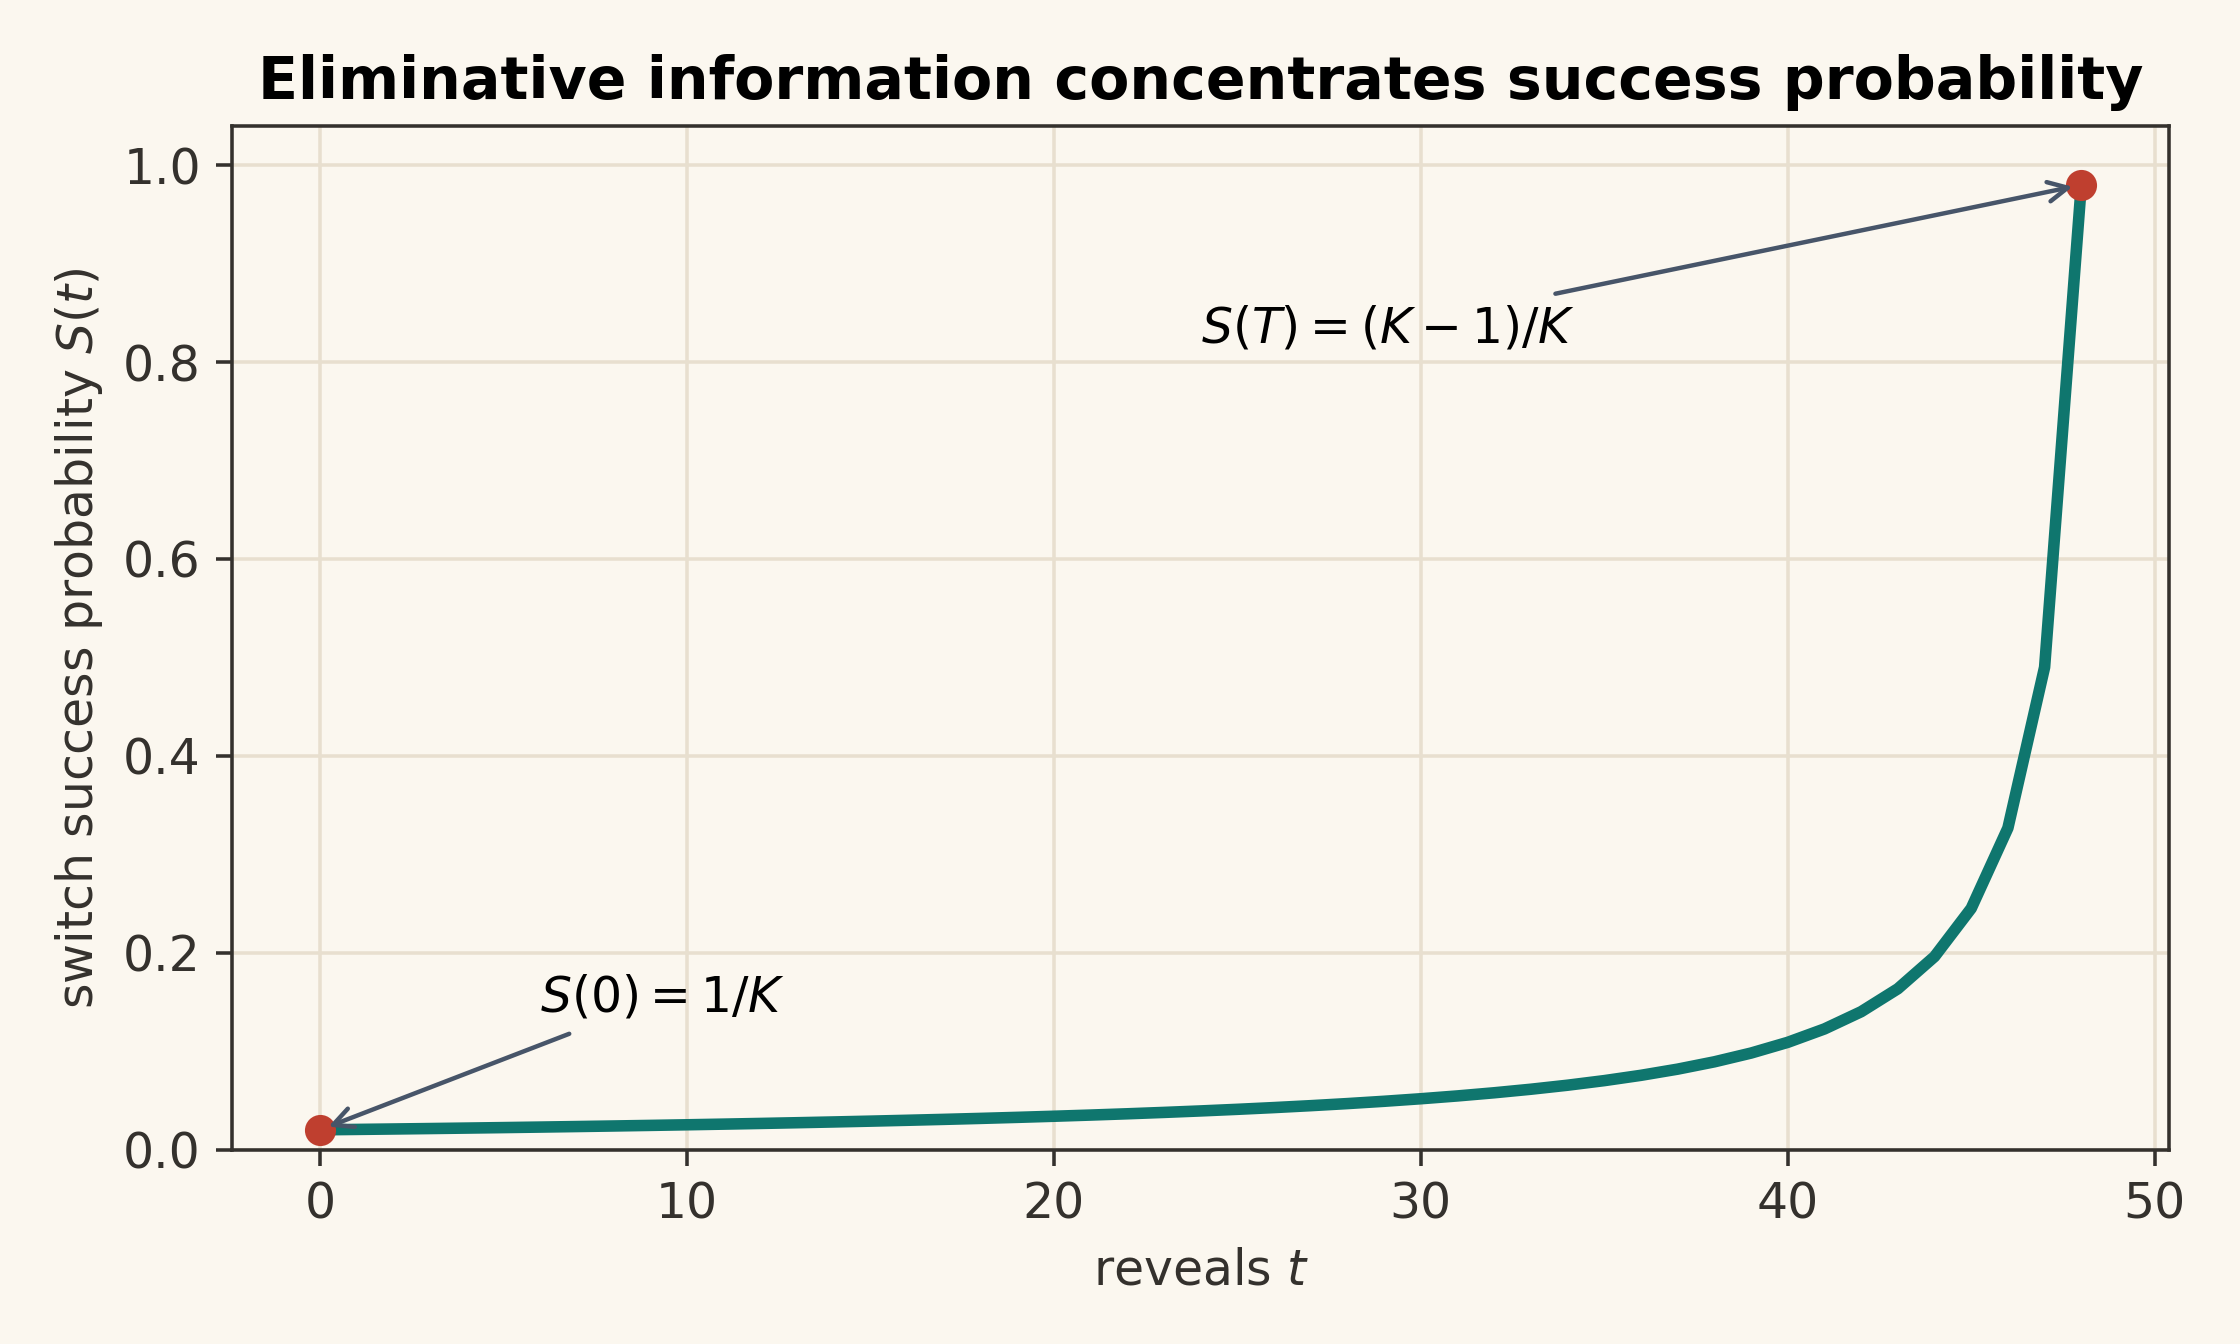
\includegraphics[width=0.86\linewidth]{fig_S.png}
  \caption{For $K=50,m=1$, switch success is almost flat early and then rises
  sharply as the last losing doors are eliminated.}
  \label{fig:S}
\end{figure}

\section{Increasing Marginal Value}

Let
\[
  \Delta_t=S(t+1)-S(t),\qquad 0\le t\le \Tmax-1.
\]

\begin{proposition}[Marginal value]
\[
  \Delta_t
  =
  \frac{m(K-1)}{K(K-2-t)(K-1-t)}.
\]
In particular, $\Delta_t$ is strictly increasing in $t$.
\end{proposition}

\begin{proof}
Subtract consecutive values:
\[
\begin{aligned}
  \Delta_t
  &=
  \frac{m(K-1)}{K(K-2-t)}
  -
  \frac{m(K-1)}{K(K-1-t)}  \\
  &=
  \frac{m(K-1)}{K(K-2-t)(K-1-t)}.
\end{aligned}
\]
The denominator decreases as $t$ increases, so the marginal value strictly
increases.
\end{proof}

\begin{figure}[ht]
  \centering
  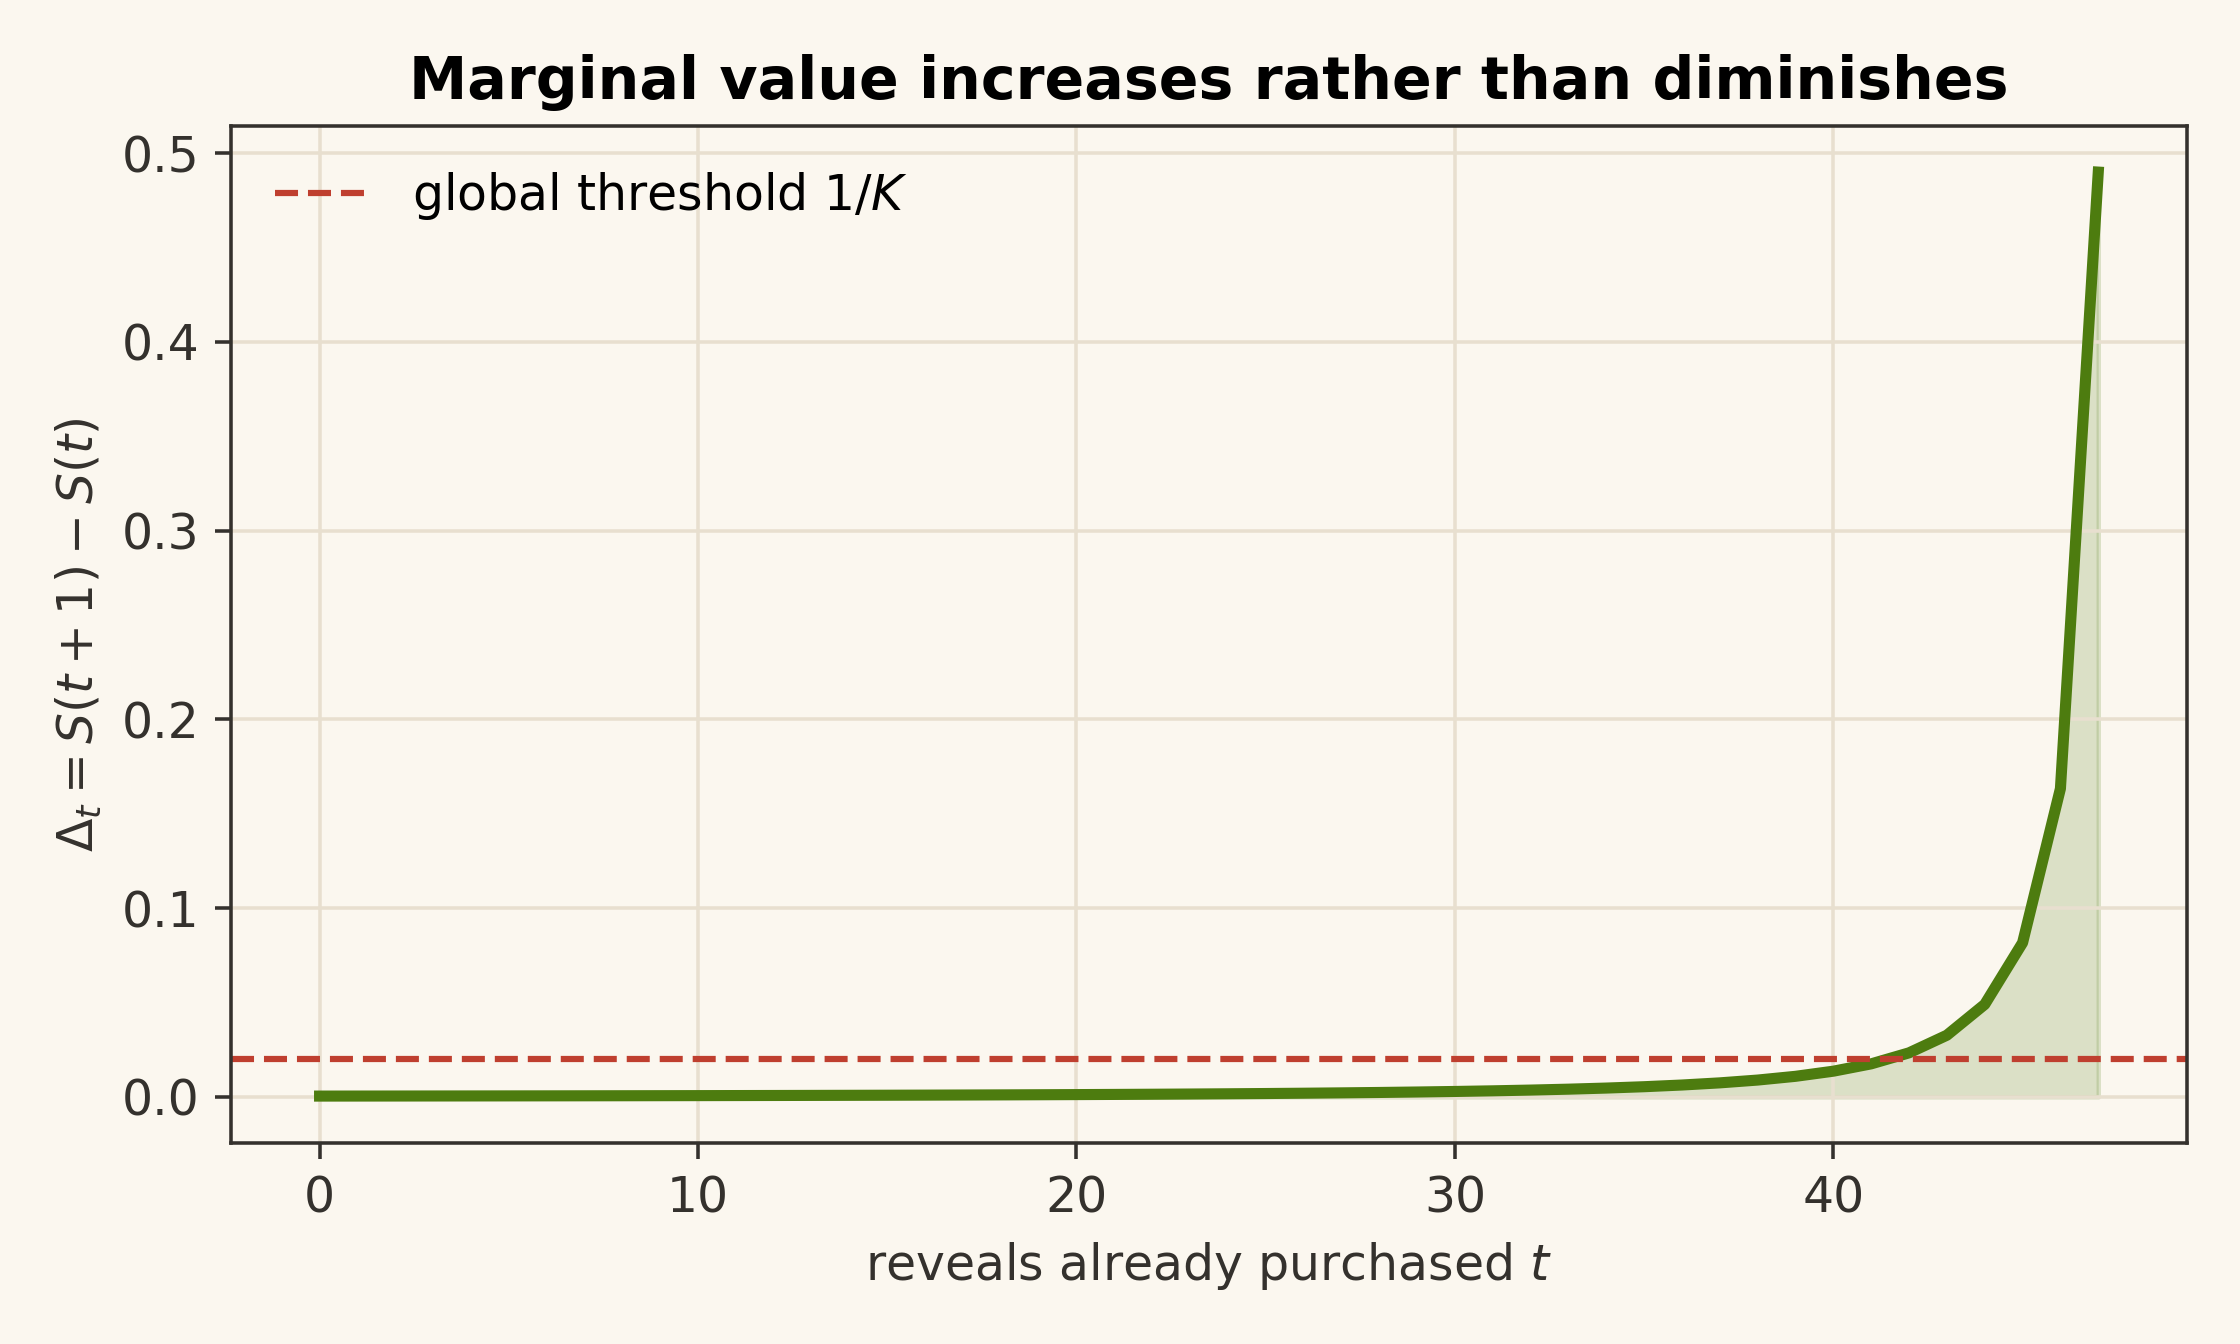
\includegraphics[width=0.86\linewidth]{fig_marginal.png}
  \caption{The marginal value of another reveal rises over time.  This is the
  opposite shape from standard diminishing-returns search models.}
  \label{fig:marginal}
\end{figure}

\section{The Costly Stopping Problem}

Suppose each reveal costs $c$, and normalize the value of a prize to $1$.
After $t$ reveals, switching has net value
\[
  W(t)=S(t)-ct.
\]
The optimal stopping problem is deterministic:
\[
  t^*\in\operatorname*{arg\,max}_{0\le t\le \Tmax} W(t).
\]

\begin{theorem}[Endpoint optimality]
The function $W(t)$ attains its maximum over
$\{0,1,\dots,\Tmax\}$ at an endpoint.  Thus every optimal policy either buys
no reveals or buys all $\Tmax$ possible reveals.
\end{theorem}

\begin{proof}
The increments of $W$ are
\[
  W(t+1)-W(t)=\Delta_t-c.
\]
Since $\Delta_t$ is strictly increasing, these increments cross zero at most
once.  Hence $W$ first decreases and then increases, or is monotone.  Such a
discrete convex sequence cannot have a strict interior maximum.  Therefore a
maximum is attained at $t=0$ or $t=\Tmax$.
\end{proof}

\begin{theorem}[Exact critical cost]
If $\Tmax=K-m-1>0$, then the endpoint comparison has the exact threshold
\[
  c^*(K)=\frac1K.
\]
More precisely,
\[
  t^*=
  \begin{cases}
  \Tmax, & c<1/K,\\
  0, & c>1/K,
  \end{cases}
\]
and both endpoints are optimal when $c=1/K$.
\end{theorem}

\begin{proof}
At zero reveals,
\[
  W(0)=S(0)=\frac{m}{K}.
\]
At full revelation, $t=\Tmax=K-m-1$, and
\[
  S(\Tmax)
  =
  \frac{m(K-1)}{K(K-1-\Tmax)}
  =
  \frac{m(K-1)}{Km}
  =
  \frac{K-1}{K}.
\]
Thus
\[
  W(\Tmax)-W(0)
  =
  \frac{K-1}{K}
  -
  \frac{m}{K}
  -
  c(K-m-1)
  =
  (K-m-1)\left(\frac1K-c\right).
\]
The sign is determined exactly by whether $c$ is below, equal to, or above
$1/K$.
\end{proof}

\begin{figure}[ht]
  \centering
  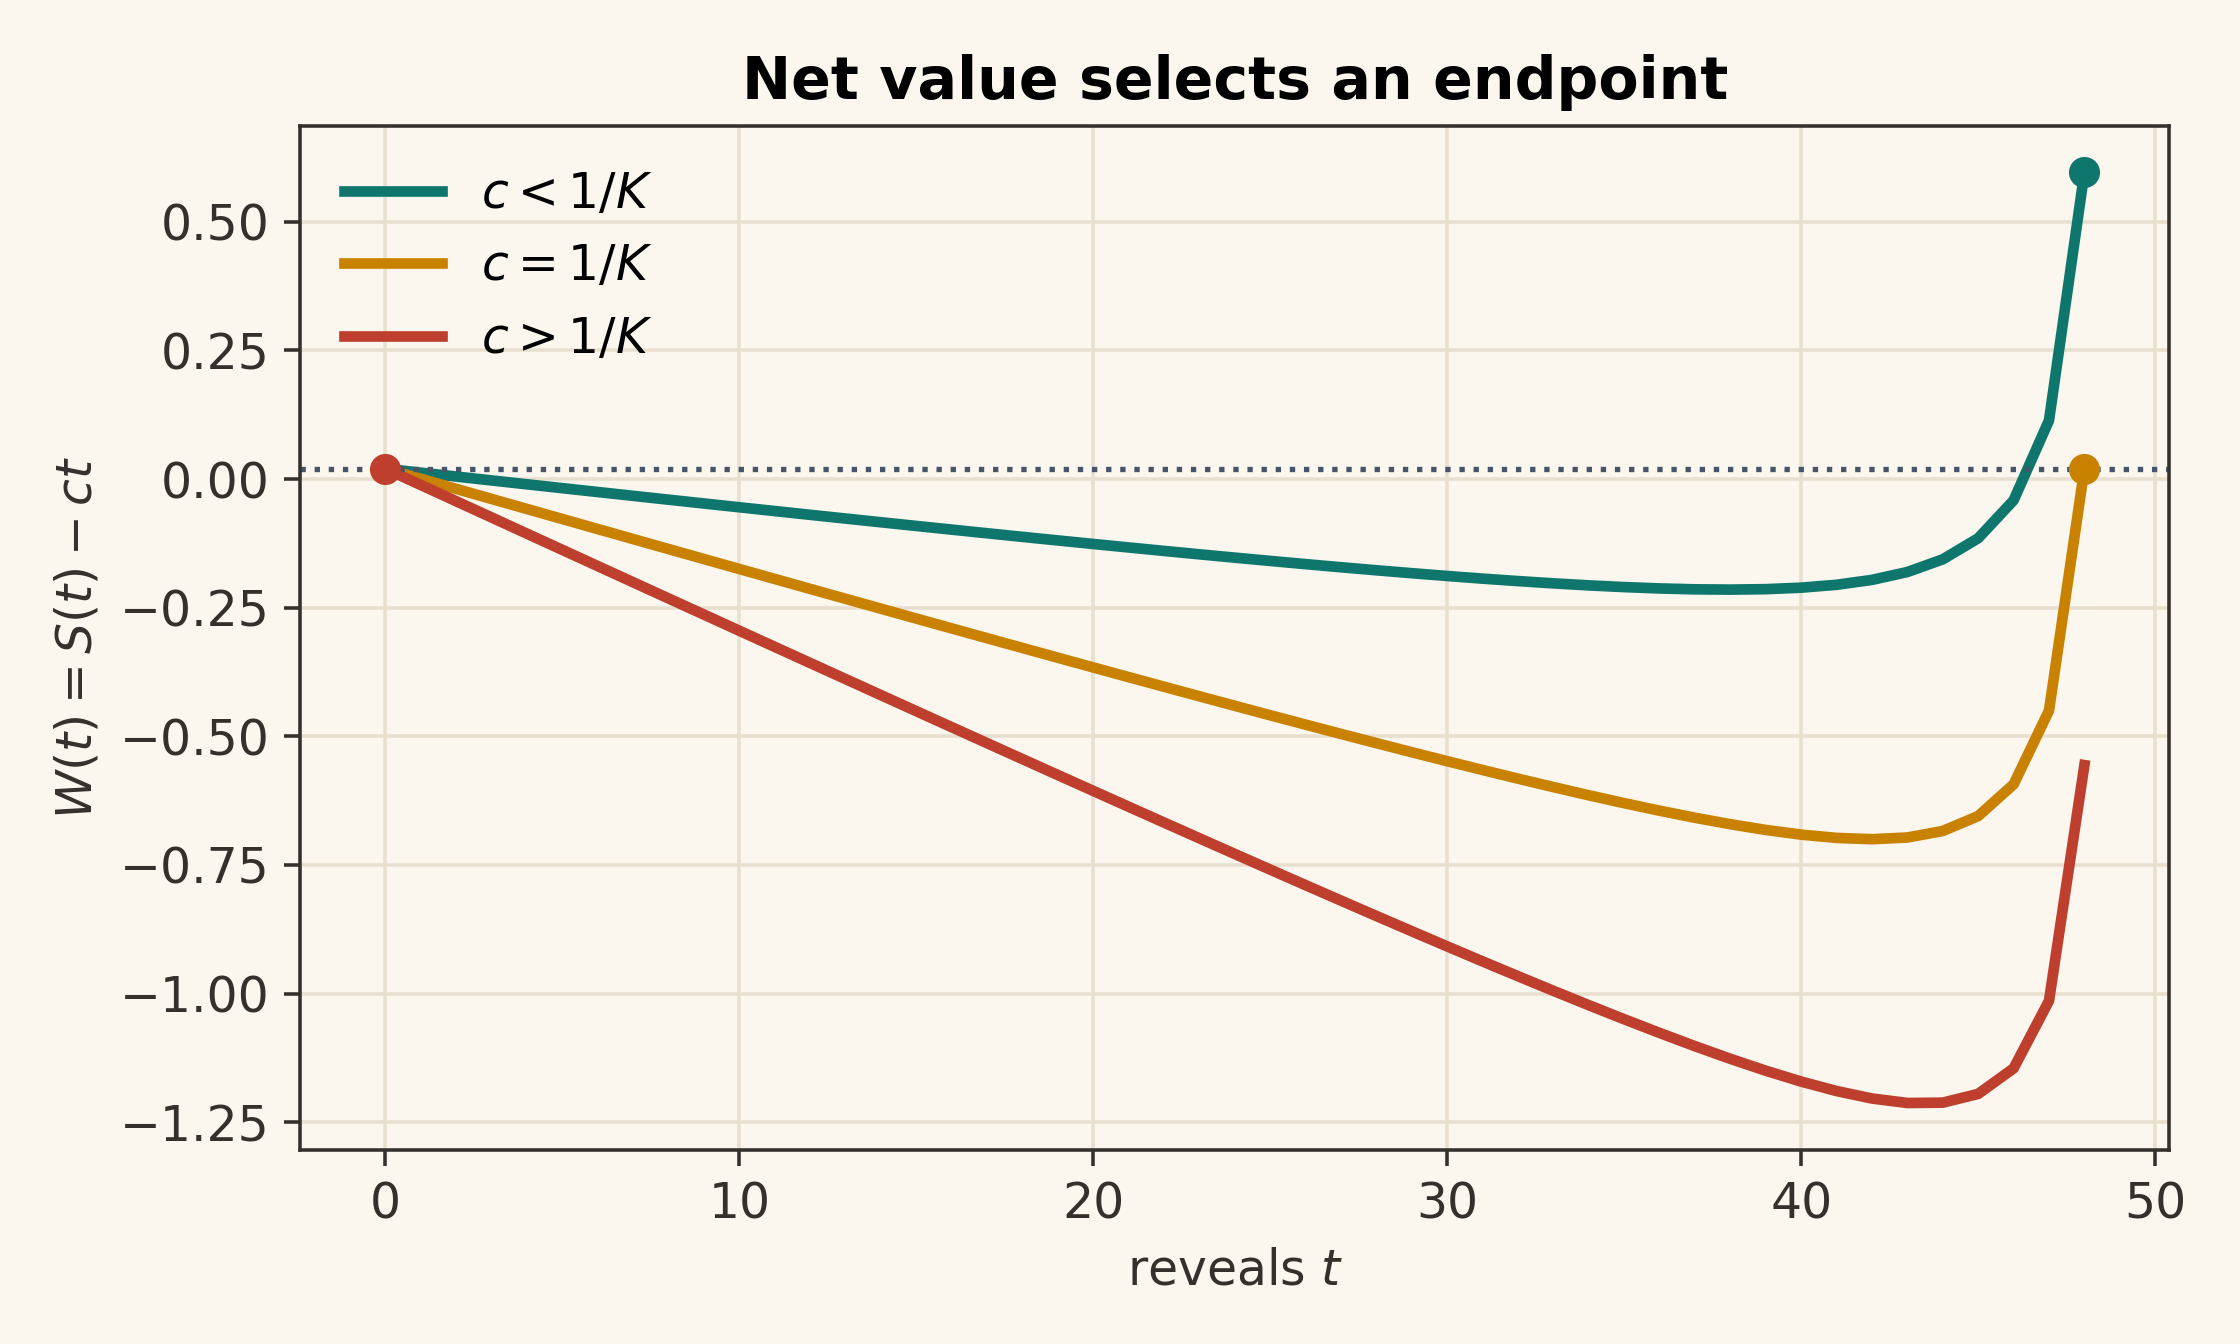
\includegraphics[width=0.86\linewidth]{fig_W.png}
  \caption{For $K=50,m=1$, net value chooses one of the two endpoints.  At
  the critical cost $c=1/K$, the endpoints tie.}
  \label{fig:W}
\end{figure}

\section{Why Myopic Search Fails}

A myopic policy buys the next reveal only if its immediate gain exceeds cost:
\[
  \Delta_t\ge c.
\]
This rule is safe in many settings with decreasing marginal value.  Here it
can be badly wrong.  For example, with $m=1$,
\[
  \Delta_0=\frac{1}{K(K-2)}
  \quad\text{but}\quad
  c^*=\frac1K.
\]
For every cost satisfying
\[
  \frac{1}{K(K-2)}<c<\frac1K,
\]
the first reveal fails the myopic test, yet the globally optimal policy buys
all reveals.  The early reveals are individually unattractive because their
purpose is to unlock the much more valuable late reveals.

\section{Numerical Illustrations}

The figures below are not needed for the proof; they make the threshold
geometry visible.

\begin{figure}[ht]
  \centering
  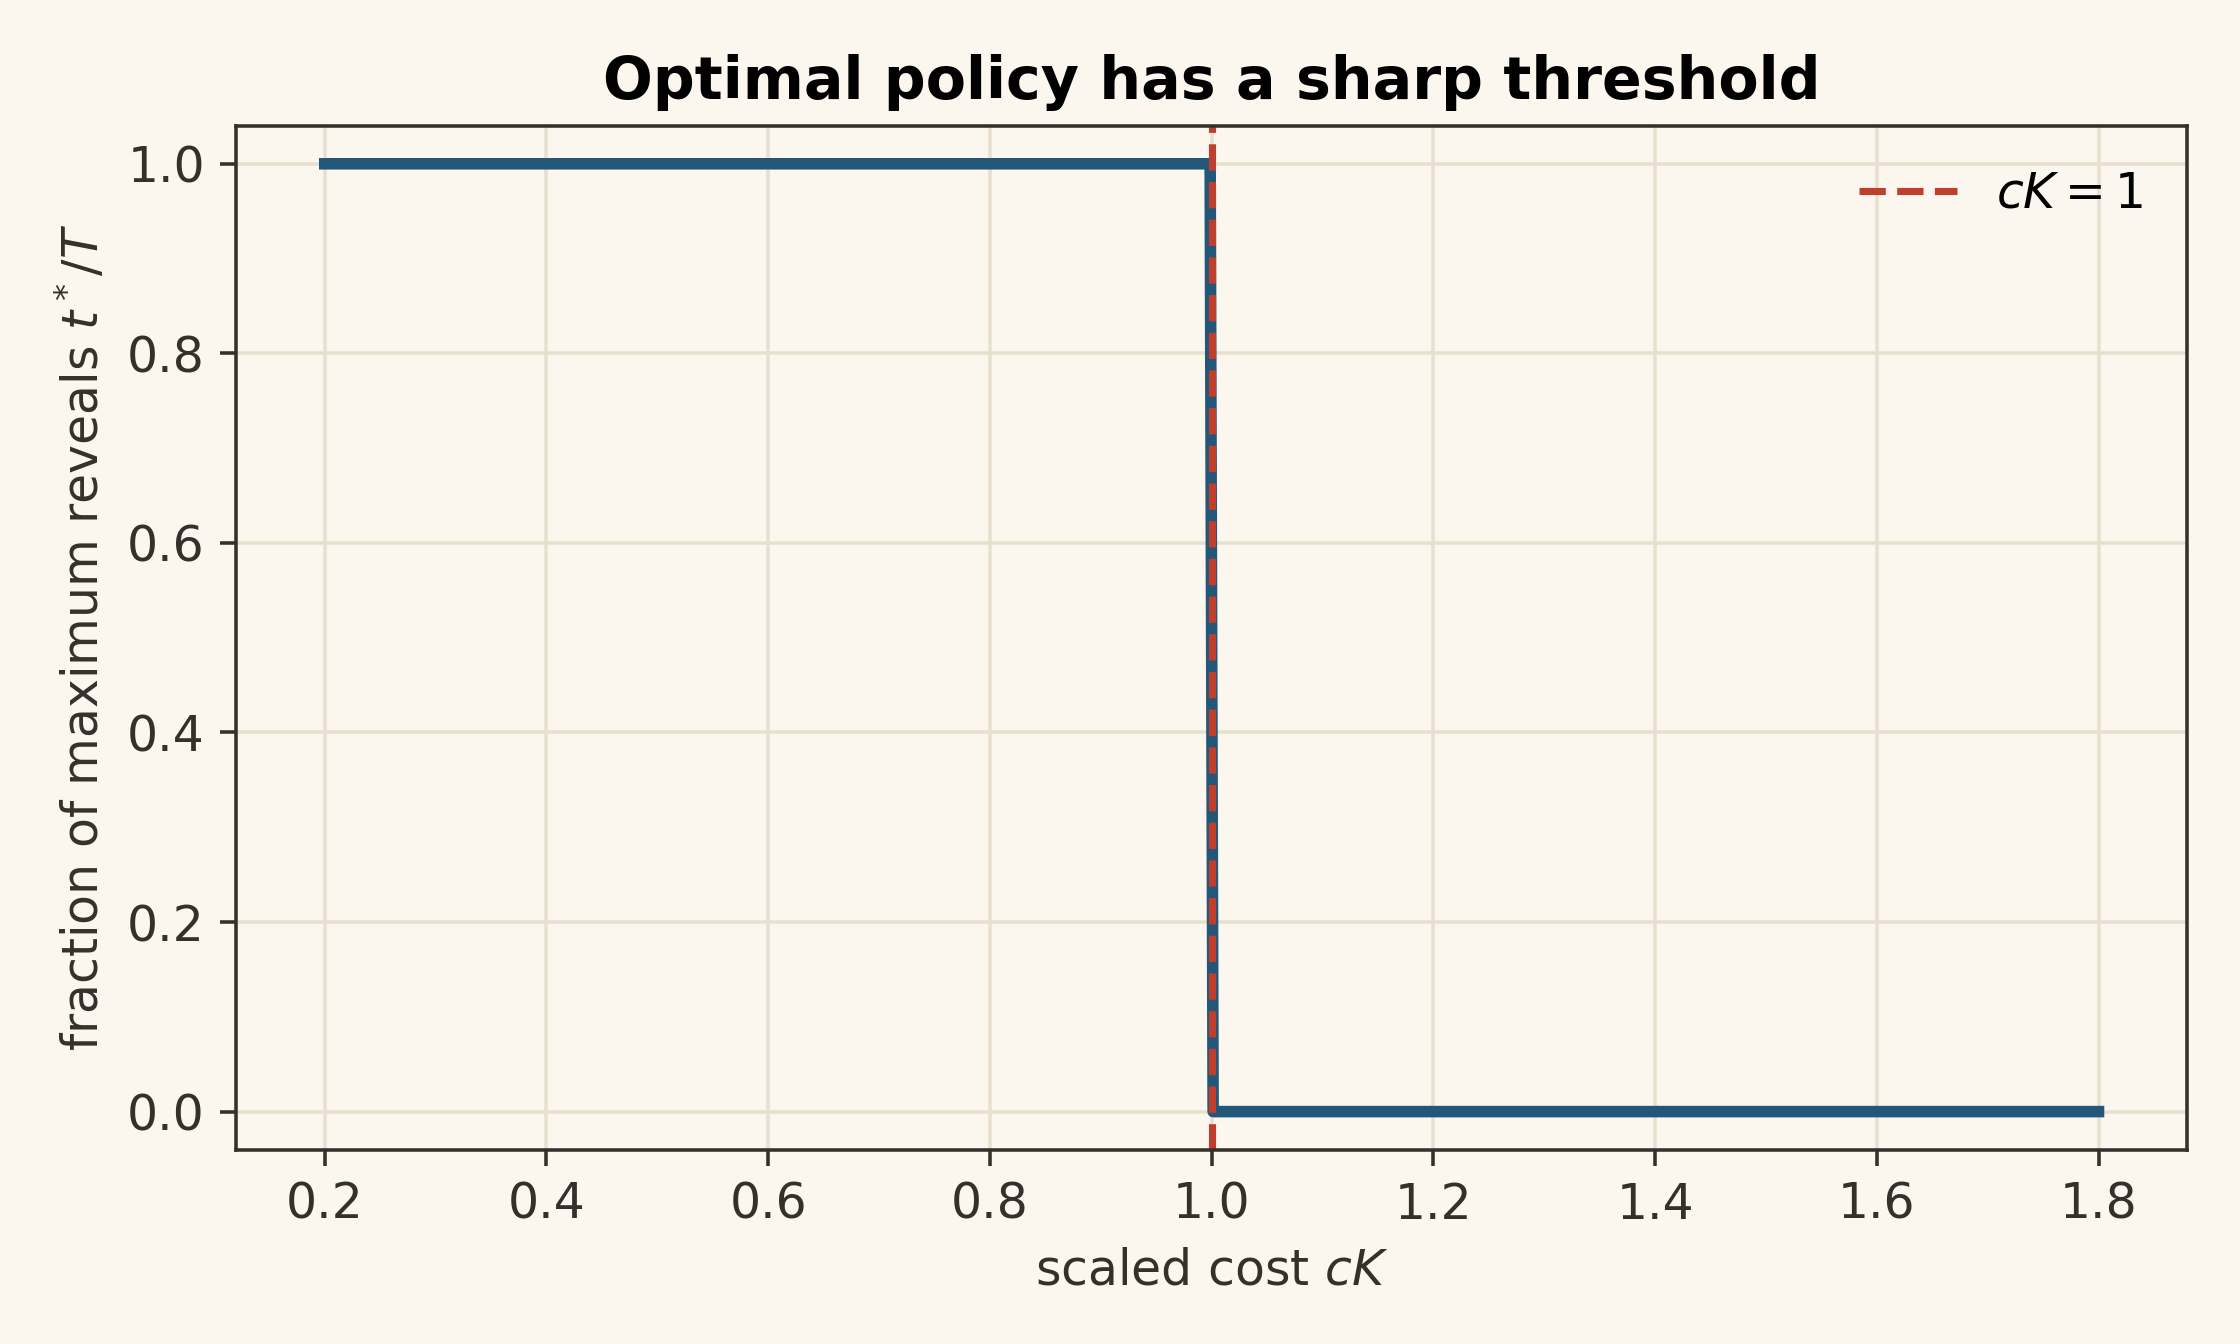
\includegraphics[width=0.86\linewidth]{fig_tstar.png}
  \caption{The optimal fraction of available reveals jumps at $cK=1$.}
  \label{fig:tstar}
\end{figure}

\begin{figure}[ht]
  \centering
  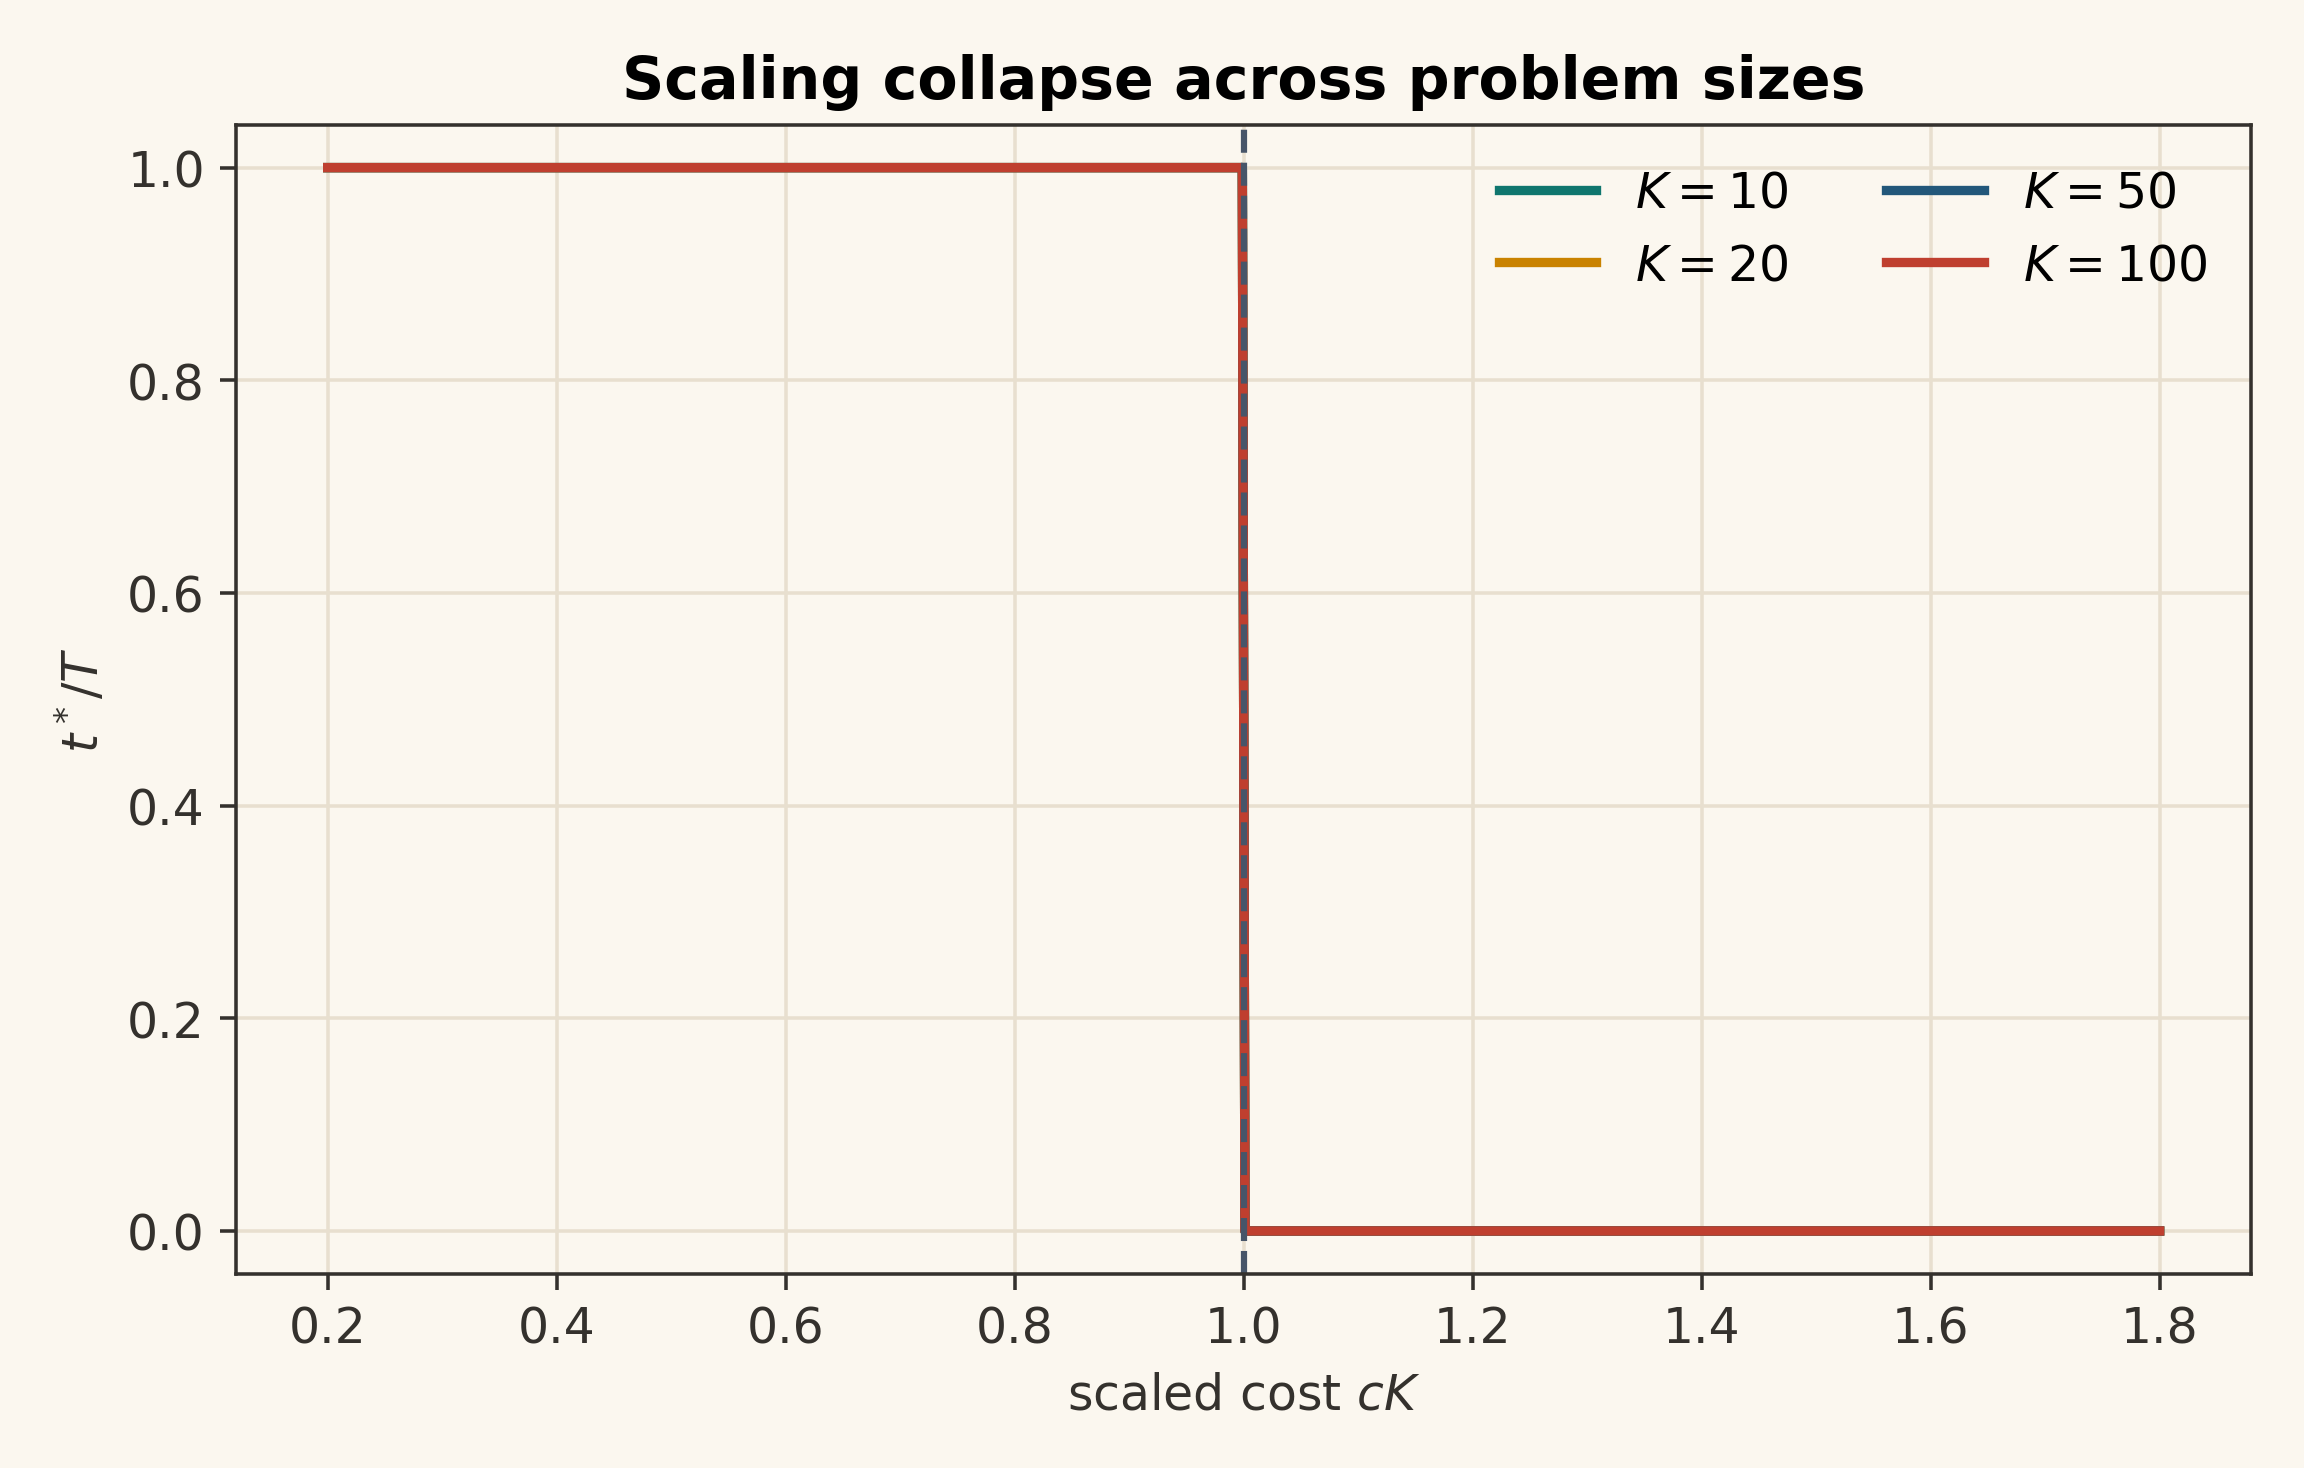
\includegraphics[width=0.86\linewidth]{fig_multiK_tstar.png}
  \caption{After scaling cost by $K$, the transition curves collapse across
  problem sizes.}
  \label{fig:multiK}
\end{figure}

\begin{figure}[ht]
  \centering
  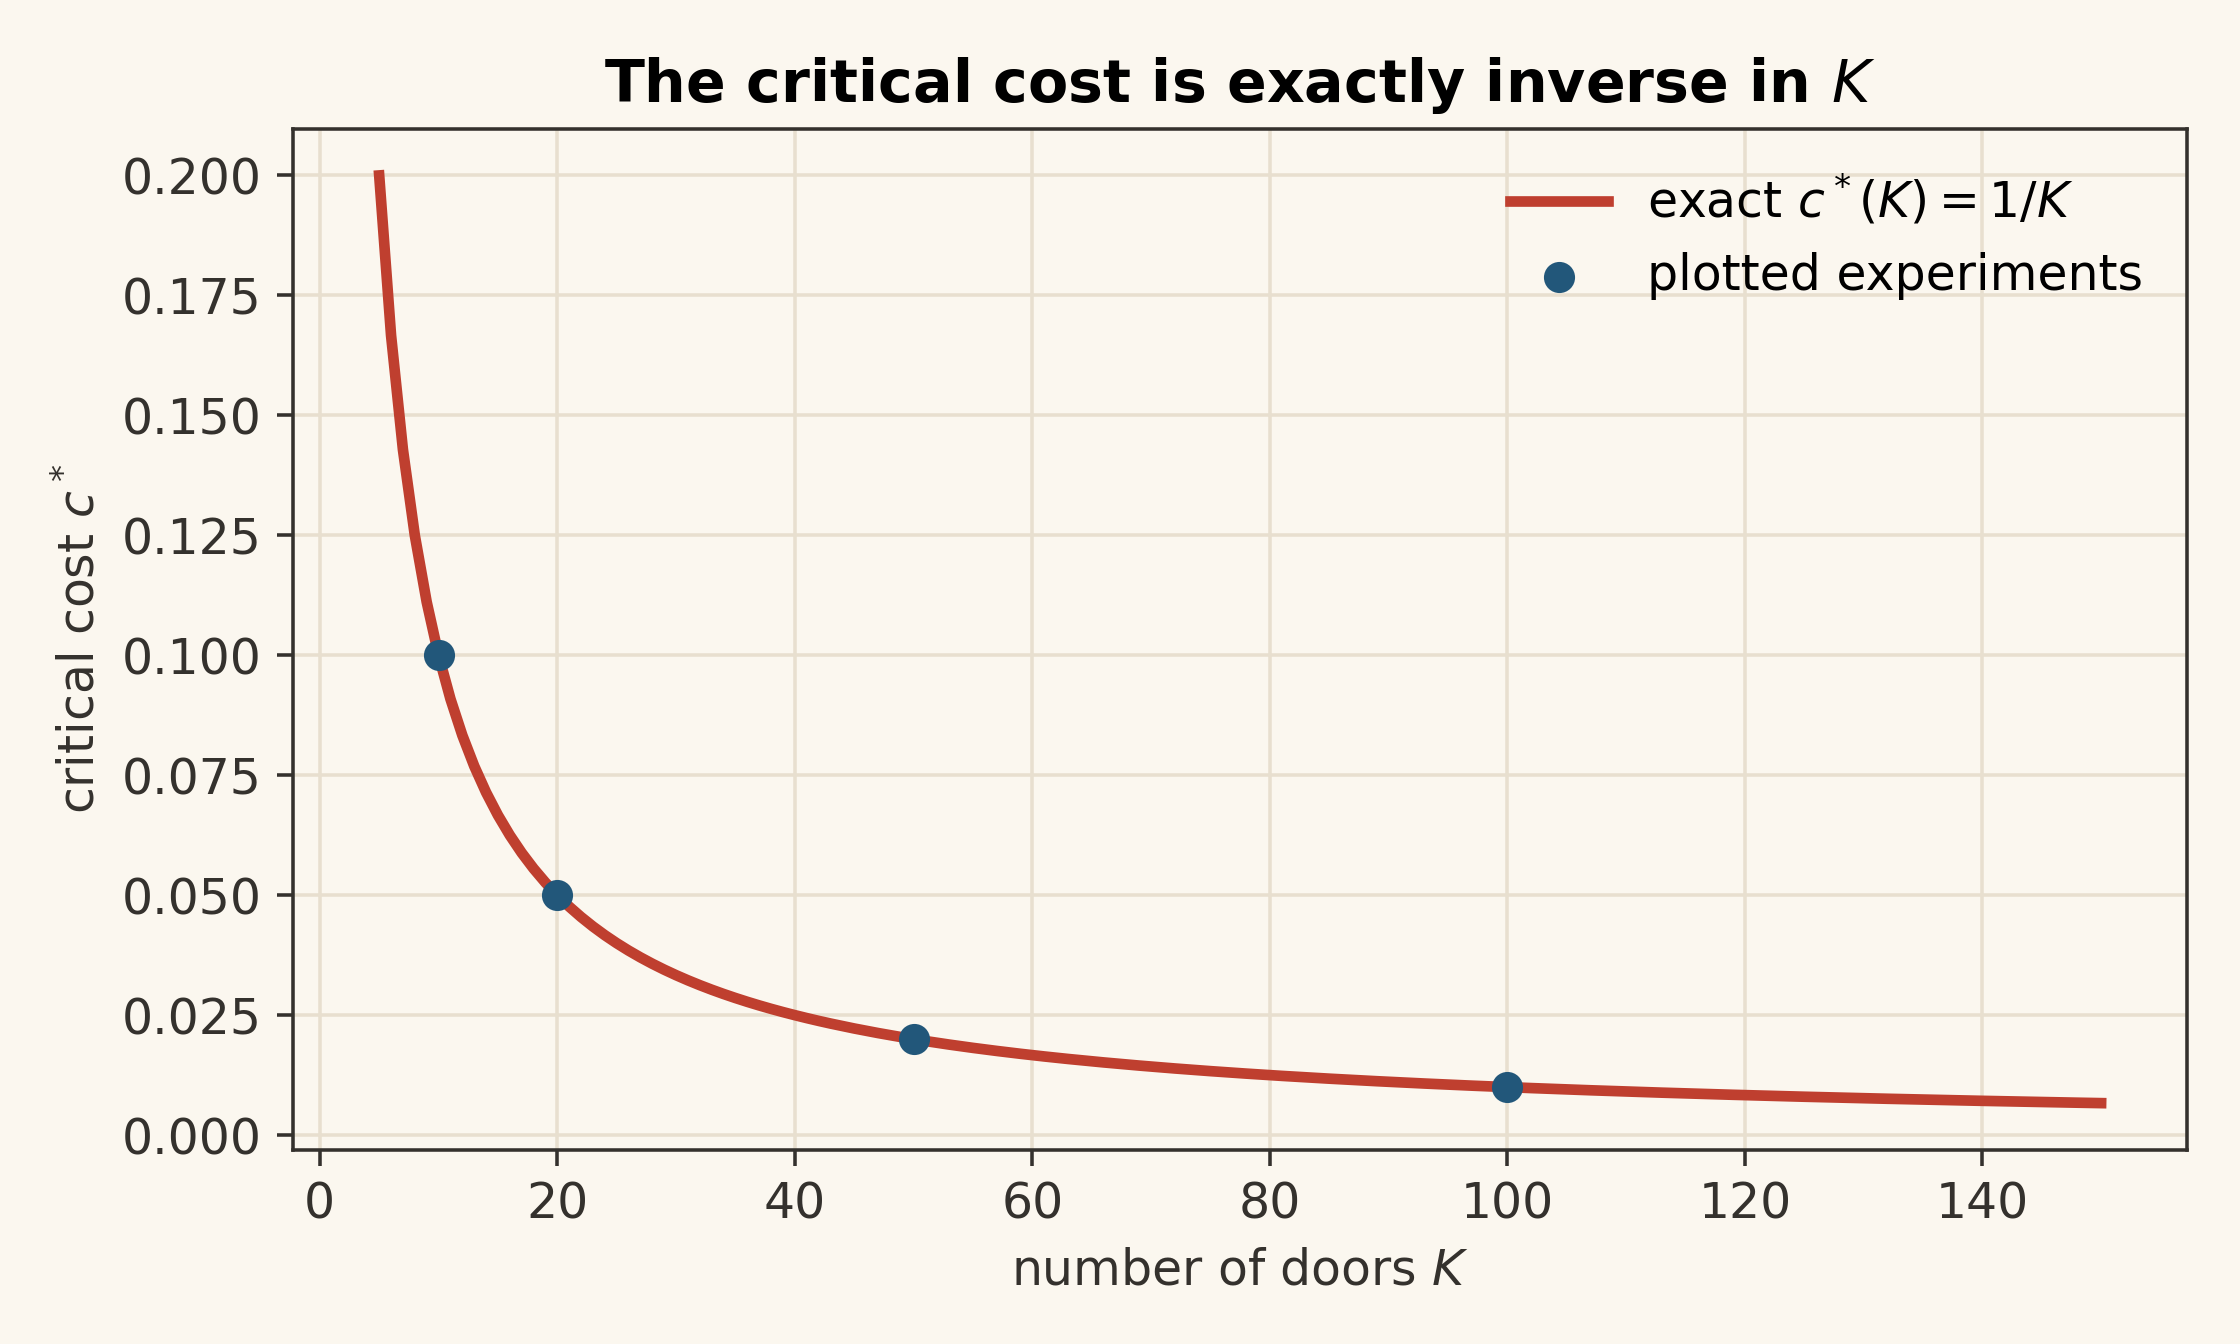
\includegraphics[width=0.86\linewidth]{fig_cstar_scaling.png}
  \caption{The critical cost is exactly $1/K$; the numerical experiments sit
  on the theoretical curve.}
  \label{fig:cstar}
\end{figure}

\section{Relation to Pandora's Box}

The problem superficially resembles Pandora's box and other sequential search
models: information is acquired over time, and stopping trades off knowledge
against cost.  The mechanism is different.

\begin{center}
\begin{tabular}{lll}
\toprule
Feature & Pandora-style search & Eliminative Monty Hall \\
\midrule
Information type & reveals sampled values & removes impossible options \\
Marginal value & typically decreasing & strictly increasing \\
Policy intuition & local indices can work & myopic rules can fail \\
Optimum shape & often interior/reservation & endpoint threshold \\
\bottomrule
\end{tabular}
\end{center}

The host's knowledge makes opened doors special: they are not random bad
draws, but certified non-prizes.  Every reveal concentrates the same hidden
probability mass over a smaller candidate set.

\section{Conclusion}

The generalized Monty Hall problem gives a compact example where information
has increasing marginal value.  The switch probability is explicit, the
stopping problem is deterministic, and the optimal policy has an exact phase
transition:
\[
  \boxed{c^*(K)=1/K.}
\]
Below this cost, one should buy every available reveal; above it, one should
buy none.  The result is a useful toy model for eliminative information: when
information removes impossibilities rather than revealing independent values,
waiting for late-stage concentration can dominate local reasoning.

\end{document}
